\documentclass[handout]{beamer}

%\usepackage{pgfpages}
%\setbeameroption{show notes}
%\setbeameroption{show notes on second screen=right}

\setbeamertemplate{caption}[numbered]

\usepackage{tikz}
\usetikzlibrary{calc, matrix, arrows, automata, shapes, positioning, shadows, trees}
\usepackage{graphicx}
\usepackage{multimedia}
\usepackage[latin1]{inputenc}
\usecolortheme{lily}
\setbeamercovered{transparent}
\usepackage{pgfplots}
\usepackage{pgfplotstable}
\usepackage{color}


\tikzset{basic/.style={draw}}
\tikzset{input/.style={basic, circle}}
\tikzset{bias/.style={basic, rectangle}}
\tikzset{neuron/.style={basic, circle}}
\tikzset{>=stealth, font=\scriptsize}
\tikzset{sectors/.style n args={2}{%
     circle, draw, minimum width=3.444em,
     append after command={%
         \pgfextra{ %
            \draw (\tikzlastnode.north) -- (\tikzlastnode.south);
            \path (\tikzlastnode.center) -- node[] {#1} (\tikzlastnode.west);
            \path (\tikzlastnode.center) -- node[] {#2} (\tikzlastnode.east);
         }
      }
   }
}


% argmax
\newcommand{\argmax}[1]{\underset{#1}{\operatorname{arg}\,\operatorname{max}}\;}

\title[\insertdate]{Nonparametric Bayes}

\author{Omar Guti\'errez}
\institute{@omargz}
\date{June 15, 2015}

\begin{document}

\begin{frame}
\titlepage
Mostly based on \textbf{A Tutorial on Bayesian Nonparametric Models} by Samuel J. Gershman.
\end{frame}
\note{
    Nothing
}

\begin{frame}
    \frametitle{Outline} 
    \tableofcontents
\end{frame}
\note{
    Nothing
}

\section{Introduction}
\begin{frame}{Introduction}
    \begin{itemize}
        \item Before to start: Statistics was already there, even before than Machine Learning (ML)
        \item What we do in ML is fitting a model to the data
        \item That is, we adjust the values of certain parameters
    \end{itemize}
\end{frame}
\note{
    \begin{itemize}
        \item Machine Learning in a nutshell
            \begin{itemize}
                \item Cloud - Internet
                \item Ubiquituos computing - IoT
                \item Eigenfaces
                \item Statistics - Data Science
                \item That is marketing :)
            \end{itemize}
    \end{itemize}
}

\begin{frame}{Linear Regression}
\begin{figure}[H]
    \centering
    \pgfmathsetseed{1138} % set the random seed
\pgfplotstableset{ % Define the equations for x and y
    create on use/x/.style={create col/expr={42+2*\pgfplotstablerow}},
    create on use/y/.style={create col/expr={(0.6*\thisrow{x}+130)+5*rand}}
}
% create a new table with 30 rows and columns x and y:
\pgfplotstablenew[columns={x,y}]{30}\loadedtable

% Calculate the regression line
\pgfplotstablecreatecol[linear regression]{regression}{\loadedtable}

\pgfplotsset{
    colored residuals/.style 2 args={
        only marks,
        scatter,
        point meta=explicit,
        colormap={redblue}{color=(#1) color=(#2)},
        error bars/y dir=minus,
        error bars/y explicit,
        error bars/draw error bar/.code 2 args={
            \pgfkeys{/pgf/fpu=true}
            \pgfmathtruncatemacro\positiveresidual{\pgfplotspointmeta<0}
            \pgfkeys{/pgf/fpu=false}
            \ifnum\positiveresidual=0
                \draw [#2] ##1 -- ##2;
            \else
                \draw [#1] ##1 -- ##2;
            \fi
        },
        /pgfplots/table/.cd,
            meta expr=(\thisrow{y}-\thisrow{regression})/abs(\thisrow{y}-\thisrow{regression}),
            y error expr=\thisrow{y}-\thisrow{regression}
    },
    colored residuals/.default={brown}{brown}
}

\begin{tikzpicture}
\begin{axis}[
xlabel=x, % label x axis
ylabel=y, % label y axis
axis lines=left, %set the position of the axes
xmin=40, xmax=105, % set the min and max values of the x-axis
ymin=150, ymax=200, % set the min and max values of the y-axis
]

\makeatletter
\addplot [colored residuals] table {\loadedtable};
\addplot [
    no markers,
    thick, black
] table [y=regression] {\loadedtable} ;
\end{axis}

\end{tikzpicture}

    \caption{Linear Regression}
\end{figure}
\end{frame}
\note{
    In linear models, we adjust the $\beta$ values
}

\begin{frame}{Neural Networks}
\begin{figure}[H]
    \centering
    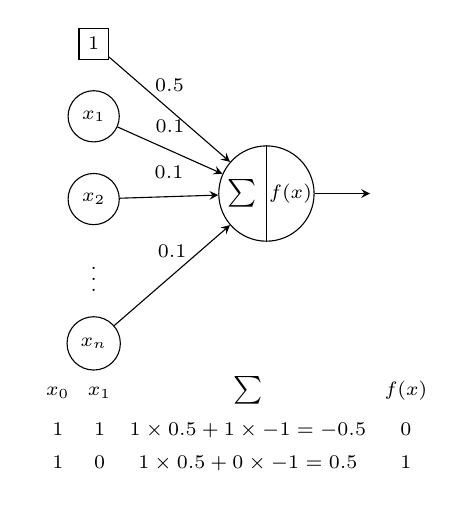
\begin{tikzpicture}[ampersand replacement=\&]

    \node[bias] (bias) {1};
    \node[input, below=1.1em of bias] (i1) {$x_1$};
    \node[input, below=1.1em of i1] (i2) {$x_2$};
    \node[below=0.55em of i2] (idots) {$\vdots$};
    \node[input, below=0.55em of idots] (in) {$x_n$};

    \node[sectors={$\sum$}{$f(x)$}, right=4.5em of bias] (sum) at ($(bias)!0.5!(in)$) {};
    \node[, right=2em of sum] (aux) {};

    \draw[->](bias) to node[above=0.3em] {$0.5$} (sum);
    \draw[->](i1) to node[above=0.3em] {$0.1$} (sum);
    \draw[->](i2) to node[above=0.3em] {$0.1$} (sum);
    \draw[->](in) to node[above=0.3em] {$0.1$} (sum);
    \draw[->](sum) -- (aux);

    \matrix[matrix of nodes, below=7.333em of in] at ($(i1)!0.5!(aux)$) {
        $x_{0}$ \& $x_{1}$ \& $\sum$                              \& $f(x)$ \\
        1       \& 1       \& $1 \times 0.5 + 1 \times -1 = -0.5$ \& 0      \\
        1       \& 0       \& $1 \times 0.5 + 0 \times -1 = 0.5$  \& 1      \\
    };

\end{tikzpicture}

    \caption{Perceptron}
\end{figure}
\end{frame}
\note{
In neural networks, we adjust the value of the weights.
}

\begin{frame}{Hidden Markov Models}
\begin{figure}[H]
    \centering
    
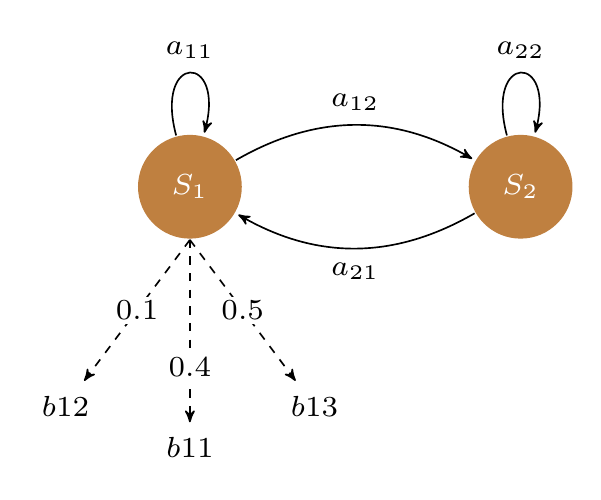
\begin{tikzpicture}[->,>=stealth',shorten >=1pt,node distance=2.8cm,
                semithick,scale=1.5,transform shape]
\tikzstyle{every state}=[fill=brown,draw=none,text=white]

\node[state]    (A)                    {$S_1$};
\node[state]    (B) [right of=A]       {$S_2$};


\path[auto] (A) edge [loop above] node {$a_{11}$} (A)
          edge [bend left]  node {$a_{12}$} (B)
      (B) edge [loop above] node {$a_{22}$} (B)
          edge [bend left]  node {$a_{21}$} (A);

\node (01) at ([shift={(-3em,-4em)}]A.south) {$b12$};
\node (04) at ([shift={(0,-5em)}]A.south) {$b11$};
\node (05) at ([shift={(3em,-4em)}]A.south) {$b13$};

\draw [shorten >=0pt,dashed] (A.south) --node[pos=.7,fill=white,inner sep=1pt]{0.4} (04);
\draw [shorten >=0pt,dashed] (A.south) --node[fill=white,inner sep=1pt]{0.1} (01);
\draw [shorten >=0pt,dashed] (A.south) --node[fill=white,inner sep=1pt]{0.5} (05);

\end{tikzpicture}

    \caption{Hidden Markov Models}
\end{figure}
\end{frame}
\note{
In HMM, we adjust the hidden states
}

\begin{frame}{Bayesian Learning}
\Huge
\begin{equation}
    \textcolor{red}{P(h|D)} =
    \frac{
    \textcolor{green}{P(D|h)}
    \textcolor{blue}{P(h)}
    }
    {\textcolor{brown}{P(D)}}
\end{equation}
\end{frame}
\note{
    \begin{itemize}
        \item And now, let's talk about the models we are concerned with
        \item The interesting facts in our datasets are governed by probabilities distributions ...
        \item by reasoning about these probabilities we can do inferences
        \item Bayesian reasoning give us a basis to manipulate probabilities
        \item Bayesian is not exactly Bayesian, is the same as if we think in we are Newtonian only because we use Calculus
        \item $P(h)$ initial probability for hypothesis $h$, prior probability, prior knowledge
        \item $P(D)$ prior probability of the trainig data
        \item $P(D|h)$ likelihood of $h$
        \item $P(h|D)$ posterior probability of ...
    \end{itemize}
}

\begin{frame}{Maximum Likelihood Estimation}
\Large
\begin{equation}
    \begin{aligned}
        h_{MAP} &\equiv \argmax {h \in H} P(h|D)\\
                &= \argmax {h \in H} \frac{P(D|h)P(h)}{P(D)}\\
                &= \argmax {h \in H} P(D|h)P(h)\\
        h_{MLE} &= \argmax {h \in H} P(D|h)
    \end{aligned}
\end{equation}
\end{frame}
\note{
    \begin{itemize}
        \item If you want to learn machine learning put this in your hearth
        \item Now we have seen the very basic idea behind Bayes reasoning...
        \item ... we will return to this later
    \end{itemize}
}

\section{Example: clustering}
\begin{frame}{Data is a mess}
    \begin{itemize}
        \item The articles in Wikipedia
        \item The species in the planet
        \item The hashtags on Twitter
    \end{itemize}
\end{frame}
\note{
Let's think in the next examples...
The data is evolving
}

\begin{frame}{How the problem is \textit{sometimes} addressed}
    \begin{itemize}
        \item Let's start with the classic approach
        \item Let's do clustering
        \item Let's use Gaussian Mixture Models (GMM)
        \item We can fit several models and then compare them with some metric.
        % add an original scatterplot
        % add an image with clusters classified
        % add an image with BIC
    \end{itemize}
\end{frame}
\note{
	\begin{itemize}
        \item We can use Gaussian Mixture Models
        \item How many classes should I use in my mixture model?
        \item Do the connection with Maximum Likelihood, EM, and GMM
        \item Do the connection with Maximum Likelihood, and linear models
        %\item Learning more from the data as we see it.
	\end{itemize}
}

\begin{frame}{How the problem is \textit{sometimes} addressed}
    {\centering
    \begin{figure}[H]
        \centering
        \includegraphics[width=0.75\textwidth, trim=4 4 4 4, clip]{code/gmm.jpg}
        \caption{Points classified with GMM}
    \end{figure}
    }
\end{frame}

\begin{frame}{How we can \textit{alternatively} approach the problem?}
    {\centering
    \begin{figure}[H]
        \includegraphics[width=0.75\textwidth, trim=10 10 10 10, clip]{code/dpgmm.jpg}
        \caption{Points classified with Infinite GMM}
    \end{figure}
    }
\end{frame}

\begin{frame}{How do we approach the problem?}
	\begin{itemize}
        \item Another interesting approach is to use Bayesian Nonparametric (BNP) models
        \item BNP models will build a model than can adapt its complexity to the data
	\end{itemize}
\end{frame}
\note{
    \begin{itemize}
        \item Learning more from the data as we see it
    \end{itemize}
}

\section{Bayesian nonparametric models}
\begin{frame}{Bayesian nonparametric models}

    \begin{figure}[H]
        \centering
        \tikzset{
  basic/.style  = {draw, text width=2cm, align=center, drop shadow, font=\sffamily\footnotesize, rectangle, fill=gray!30},
  root/.style   = {basic, rounded corners=2pt, thin},
  level 2/.style = {basic, rounded corners=6pt, thin, text width=6em},
  level 3/.style = {basic, rounded corners=2pt, thin, text width=5em},
  level 4/.style = {basic, rounded corners=2pt, thin, text width=6em, font=\tiny}
}

\begin{tikzpicture}[
  level 1/.style={sibling distance=40mm},
  edge from parent/.style={->,draw},
  edge from node/.style={->,draw, black},
  >=latex]

% root of the the initial tree, level 1
\node[root] {\textbf{Bayesian models}}
% The first level, as children of the initial tree
  child {node[level 2] (c1) {Parametric}}
  child {node[level 2] (c2) {\textbf{Nonparametric}}
    child {node[level 3] (c21) {\textbf{Mixture}}
        child {node[level 4] (c211) {\textbf{Chinese Restaurant\\ Process}}}
    }
    child {node[level 3] (c22) {Latent factor}
        child {node[level 4] (c221) {Indian Buffet\\ Process}}
    }
  };

\node (comment) [above left = of c1] {Finite};
    \draw [->, thick] (comment) to [in = 110] (c1);

\node (comment2) [above right = of c2] {Infinite};
    \draw [->, thick] (comment2) to [in = 110] (c2);

\node (comment2) [above right = of c2] {Infinite};
    \draw [->, thick] (comment2) to [in = 110] (c2);

\node (comment3) [below left = of c211] {Dirichlet Processes!};
    \draw [->, thick] (comment3) to [in = 211] (c211);
    \draw [->, thick] (comment3) to [in = 221] (c221);

\end{tikzpicture}

    \end{figure}

\end{frame}

\begin{frame}{Recap: Bayesian parametric vs nonparametric models}
    \begin{itemize}
        \item Traditional approach (finite)
           \begin{itemize}
               \item The number of parameters $\theta$ (e.g. clusters) is prespecified
               \item We have a prior distribution over parameters $P(\theta)$
               \item For example, in the Gaussian mixture model, each cluster will be modelled
                   using a parametric model (e. g. Gaussian)
           \end{itemize}
        \item Bayesian nonparametric models
           \begin{itemize}
               \item We assume that there is an \textbf{infinite} number of latent clusters
               \item A finite number of clusters is \textit{inferred} from data
               \item The number of clusters grow as new data points are observed
           \end{itemize}
    \end{itemize}
\end{frame}


\section{Chinese Restaurant Process}
\begin{frame}{Chinese Restaurant Process}
    {\centering
    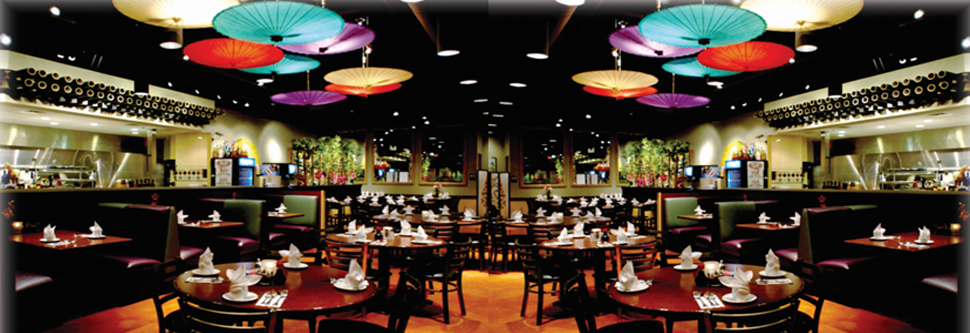
\includegraphics[width=0.75\textwidth]{figures/crp.png}\par
    }
    \pause

    \begin{itemize}
        \item Imagine a restaurant with an infinite number of tables,
        \item and a sequence of customers entering the restaurant and sitting down.
        \item The first customer enters and sits at the first table
        \item The second customer enters and sits...
            \begin{itemize}
                \item at the first table with probability $\frac{1}{1 + \alpha}$
                \item at the second table with probability $\frac{\alpha}{1 + \alpha}$
            \end{itemize}
        \item We realize that CRP is a form of clustering: $K$ groups and each group with size $N_k$
    \end{itemize}
\end{frame}

%\section{Bayesian Inference}
%\begin{frame}{Bayesian Inference}
%	\begin{itemize}
%        \item $P(A|D) \propto P(D|A) P(A)$
%	\end{itemize}
%\end{frame}

%\section{Generative Model}
%\begin{frame}{Generative Model}
%	\begin{itemize}
%        \item *
%	\end{itemize}
%\end{frame}


%\section{Python}
%\begin{frame}{Python}
%	\begin{itemize}
%        \item *
%	\end{itemize}
%\end{frame}

%\section{Beta and Dirichlet Distribution}
%\begin{frame}{Dirichlet Distribution}
%    \begin{itemize}
%        \item $\beta$ distribution.
%        \item Dirichlet distribution is a generalization of $\beta$ distribution.
%    \end{itemize}
%\end{frame}

\begin{frame}{What else?}
    \begin{itemize}
        %\item $\beta$ distribution.
        \item Dirichlet distribution is a generalization of $\beta$ distribution.
        \item Dirichlet process
    \end{itemize}
\end{frame}

\begin{frame}
\huge{Thank you}\\
\huge{Questions?}\\
\end{frame}

\end{document}
